\documentclass{article}
\usepackage[utf8]{inputenc}

\usepackage{tikz}
\usetikzlibrary{positioning, fit, arrows}

\usepackage{geometry}
\geometry{
margin=10mm,
}

\begin{document}

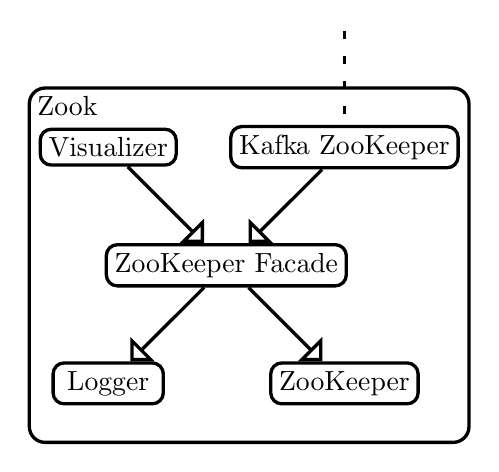
\begin{tikzpicture}[ % has a lot of options; consult the pgf manual
bend angle=15,
long_square/.style={rectangle, draw=black, fill=white, very thick, inner sep=3pt, minimum width=14mm},
rounded_square/.style={rectangle, rounded corners, draw=black, fill=white, very thick, inner sep=3pt, minimum width=14mm},
empty_circle/.style={rectangle, rounded corners=2mm, draw=black, fill=white, very thick, minimum size=4mm},
point/.style={circle, inner sep=0mm},
fit_square/.style={rectangle, rounded corners=2mm, draw=black, very thick, minimum height=45mm},
both_arrow/.style={<->, very thick},
out_arrow/.style={->, very thick},
out_hollow_arrow/.style={-open triangle 90, very thick},
in_arrow/.style={<-, very thick},
dashed_line/.style={loosely dashed, very thick},
above_edge_text/.style={above, midway, sloped},
]

\node[point](external) at (3,1.5) {};

\node[rounded_square](visualizer) at (0,0) {Visualizer};
\node[rounded_square](zk_kafka) at (3,0) {Kafka ZooKeeper};

\node[rounded_square](zk_facade) at (1.5,-1.5) {ZooKeeper Facade};

\node[rounded_square](logger) at (0,-3) {Logger};
\node[rounded_square](zk) at (3,-3) {ZooKeeper};

\node[fit_square, fit=(zk_kafka) (visualizer) (zk_facade) (logger) (zk)] (zookeeper_client) {};
\node[anchor=north west] at (zookeeper_client.north west) {Zook};



\draw[dashed_line](external) to [] node[auto]{} (zk_kafka);

\draw[out_hollow_arrow](visualizer) to [] node[auto]{} (zk_facade);
\draw[out_hollow_arrow](zk_kafka) to [] node[auto]{} (zk_facade);

\draw[out_hollow_arrow](zk_facade) to [] node[auto]{} (logger);
\draw[out_hollow_arrow](zk_facade) to [] node[auto]{} (zk);

\end{tikzpicture}

\end{document}
